\section{Features for VAD}
The first step in any automatic voice activity detection system is the extraction of acoustic features from the signal \cite{ishizuka2010noise,cho2011enhanced}.
Most techniques assume that these features are statistically stationary over the interval of a few milliseconds \cite{ishizuka2010noise}.
Thus, the speech signal is divided into short overlapping segments of fixed duration using a sliding window technique, which are then treated as `frames' of observation for feature extraction.

%TODO: introduce the frame $\vt{x}_k$ and the windowing procedure here.

%Formally, if the time-series speech signal $x[n]$ is divided into $N$ frames $\{\vt{x}_k\}_1^N$, $\vt{x}_k \in \realnumber^{N_w}$ where $N_w$ is the window size, the feature extraction problem is to find a transformation $F$ which maps every frame $\vt{x}_k$ to a lower-dimension feature vector $\vt{y}_k \in \realnumber^P$, which can capture the statistics of speech. \emph{TODO: revise this paragraph.}

The choice of features is a critical design in any classification problem.
In the voice activity detection context, good features must possess the following crucial properties:

%\begin{flushleft}
\begin{description}
    \item[Discriminative power] which measures the separateness between the distributions of noisy speech frames and noise only frames. Theoretically, a good feature should take no overlapping values between difference classes.
    \item[Noise robustness] which ensures the performance of the classifier in real-world applications, where ambiance noise might corrupt the speech signal greatly thus reduce the discriminative power of the extracted features.
\end{description}
%\end{flushleft}

There have been many features proposed in the literature, which can be broadly categorized as follow:
\begin{itemize}\addtolength{\itemsep}{-0.5\baselineskip}
	\item Energy-based features  %which derive from the energy function to detect the changes in the loudness of the signal.
	\item Spectral-domain features  %which rely on the analysis techniques in the spectral domain.
	\item Cepstral-domain features  %which rely on the analysis techniques in the cepstral domain.
	\item Harmonicity-based features  %which rely on the harmonic nature of voiced speech for detection.
	\item Long-term features  %which exploit the temporal information spread across the speech frames.
\end{itemize}
The following subsections reviews each feature category in details.
%\cite{benyassine1997robust}

\subsection{Energy-based features}
Energy is a simple measure of the loudness of the signal.
A na\"\i ve method for VAD can assume that speech is always louder than background noise, and then assign the high-energy frames to speech and lower ones to noise.
However, when the loudness of speech and noise are of similar levels, for example due to the increasing white noise in the environment or during soft speech segments, the simple energy feature fails to discriminate speech and noise.
Earlier work on VAD exploited the energies across different sub-bands to increase the discriminative power \cite{woo2000robust,benyassine1997robust}.
For example, examining the spectrums of speech and noise shows that voiced speech has high energy in the low frequency bands (below 2 kHz) and unvoiced speech is more active in the high frequency bands (either 2--4 kHz or above 4 kHz), while white noise spreads its energy equally across the entire spectrum.
Another way to improve noise robustness is to combine energy-based features with other features, such as zero-crossing rate (ZCR) \cite{rabiner1975algorithm,cho2011enhanced}, or the line spectral frequency (LSF) \cite{benyassine1997robust}.

These measures are formally defined as follow:
\begin{align}
    \operatorname*{Energy}(\vt{x}_k) & = \sum_{i=1}^{N_w} x_{k,i}^2   \\
    \operatorname*{ZCR}(\vt{x}_k) & = \sum_{i=1}^{N_w} \lvert\sgn{x_{k,i+1}} - \sgn{x_{k,i}}\rvert
\end{align}

Generally, these features work well with clean speech or high SNR conditions.
However, under considerable noise level such as when SNR falls below 10dB, their discriminative power drops drastically.
Nevertheless, with their low computation complexity, energy-based features are still employed by some standards and various real-world applications.
A typical example is the ITU-T Recommendation G.729 Annex B \cite{benyassine1997robust}, which employs a vector of features including full-band energy, zero-crossing rate and low-band (0 to 1 kHz) energy.
This standard remains the most cited work and still being used as the baseline system for performance comparison in many research.
In \cite{cho2011enhanced}, energy-based VAD is used as a preliminary event detector for further classification in an always-listening speech application.

\subsection{Spectral-domain features}
One of the most common speech processing techniques is the frequency spectrum analysis, which describes the frequency content of the signal over time \cite{rabiner1978digital}.
This is made possible by the development of the Fast Fourier Transform (FFT) algorithm.
Let $X_k \in \complexnumber^L$ be the vector of coefficients resulting from applying the $L$-point FFT on frame $\vt{x}_k$.
\begin{align}
%    \mathcal{F} \colon \realnumber^P \to \complexnumber^L \\
%    X_k = \mathcal{F}(\vt{x}_k) \\
%    X(n,\omega_k) = \sum_{l=(n-1)N_{sh}+1}^{N_w+(n-1)N_{sh}} w(l-(n-1)N_{sh}-1)x(l)e^{-j\omega_k l}
    X_{k,w} = \sum_{n=1}^N x_{k,n}e^{-j\frac{2\pi}{N}wn}
\end{align}

In the voice activity detection context, there have been many features derived from the spectral domain, many of which rely on some form of noise power estimation and subtraction \cite{boll1979suppression}:
\begin{equation}
    |\hat{X}_k|^2 = |X_k|^2 - |N|^2
\end{equation}
where $|\hat{X}_k|^2$ is the estimated clean speech power spectrum, $|X_k|^2$ is the observed noisy speech power spectrum, and $|N|^2$ is the estimated noise power spectrum. This is a simple yet efficient method to reduce the effects of additive noise in speech signal. It works by assuming that the noise component is additive and independent from speech in the power spectrum domain. Typically, this approach is coupled with the process of noise estimation, which can be achieved through training data or by averaging the long-term spectrum of the signal \cite{ramirez2004efficient,renevey2001entropy}. The techniques related to noise estimation and spectral subtraction are, in fact, the heart of \emph{speech enhancement} problem, which is a related research field. They are sometimes included in VAD systems either explicitly in a pre-processing step \cite{ramirez2004voice}, or implicitly in the feature extraction step itself \cite{ramirez2004efficient,fukuda2010long}.

%Some work derived features from the spectral envelope, or the shape of the observation frame in spectral domain \cite{Marzinzik_speechpause_2002}.

To increase the discriminative power of the features under noisy condition, many approaches consider the relative power of speech over the estimated noise across the different frequency bands of the spectrum \cite{ramirez2004efficient}. Effectively, this is equivalent to estimating the sub-band SNR's of the speech signal. In fact, even under very noisy condition (SNR=0 dB, \fig{spectrum_snr0_whitenoise}), it can be observed from the spectrum that the power of the speech signal is still distinguishable from noise in some frequency bands.

\begin{figure}[hh] %[hb] to put it to the bottom of the page
    \centering
    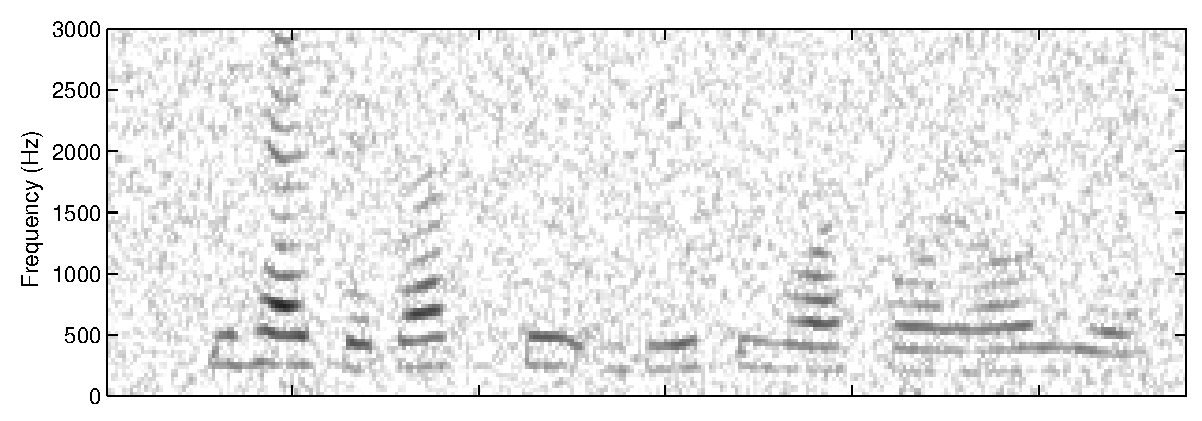
\includegraphics [scale=.6]{spectrum_snr0_whitenoise.eps}            %Adjust width to taste
    \caption[A sample spectrum of speech corrupted by white noise at SNR=0dB]{A sample spectrum of speech corrupted by white noise at SNR=0dB}
    \label{Fig:spectrum_snr0_whitenoise}        %For referencing in the text
\end{figure}

To exploit this idea, Ramirez \etal \cite{ramirez2004efficient} estimate the long-term upper bounding envelope of the spectrum over a set of $(2M+1)$ contiguous frames, and then calculate the sum of all $L$ sub-band SNRs, where $M$ is the number of neighbour frames to include in the envelope estimation, and $L$ is the number of FFT coefficients. The measure is called long-term spectral diversion, whose formulation is as follow:
\begin{equation}\label{eq:LTSD}
    \operatorname{LTSD}(X_k) = 10\log_{10} \left(\reci{L} \sum_{i=1}^{L} \frac{|\tilde{X}_{k,i}|^2}{|N_i|^2}\right)
\end{equation}
where $N_i$ is the $i$-th coefficient of the average noise spectrum, and $\tilde{X}_k = [\tilde{X}_{k,1} \dots \tilde{X}_{k,L}]^T$ is the estimated spectral envelope of the neighboring $(2M+1)$ frames:
\begin{equation}\label{eq:LTSE}
    \tilde{X}_{k,i} = \max \lbrace X_{k-M,i},\dots,X_{k,i},\dots,X_{k+M,i} \rbrace
\end{equation}

The drawback of this method, as of with any method that relies on the estimation of noise, is that its performance is sensitive to the accuracy of the noise estimation process.
In environments containing non-stationary noise, the estimation by averaging method fails to update the quickly changing characteristics of noise, causing the performance of the VAD system to drop greatly \cite{?}.

%Some work has tried to reduced the dependency on noise estimation.



\subsection{Cepstral-domain features}
Another class of features use a collection of nonlinear techniques known as cepstral analysis.
The power cepstrum is defined as the power of the Fourier transform of the log-power spectrum.
\begin{equation}
    \vt{c}_k = \left| \mathcal{F}\left(\log |X_k|^2 \right) \right|^2
\end{equation}

In a sense, this can be viewed as the `power spectrum of the log-power spectrum', which can be used to analyze the power spectrum of the signal.
Thus, cepstral features are widely used in speech recognition research \cite{rabiner1978digital}.
For VAD, the cepstral peaks can be used to determine the fundamental frequency of the speech signal \cite{rabiner1978digital,noll1967cepstrum,ahmadi1999cepstrum} (\fig{DFT_voiced_frame_clean}).
This problem is often referred to as \emph{pitch estimation}, which is another related research field of speech processing and will be discussed more in the next subsection.

%The power cepstrum has a strong peak corresponding to the pitch period of the voiced-speech segments of the signal \cite{Noll1967cepstrum}. In \cite{Ahmadi1999cepstrum}, the authors improved the


\begin{figure}[hh] %[hb] to put it to the bottom of the page, ht=top, hh=here
    \centering
    \subfloat[Log-spectrum]{\label{Fig:logspectrum_voiced}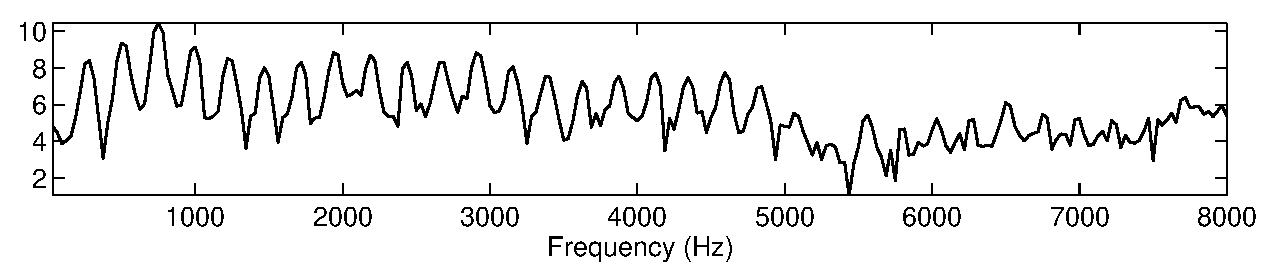
\includegraphics[scale=.6]{DFT_voiced_frame_clean.eps}} \\
%    \vspace{8mm}
    \subfloat[Cepstrum]{\label{Fig:cepstrum_voiced}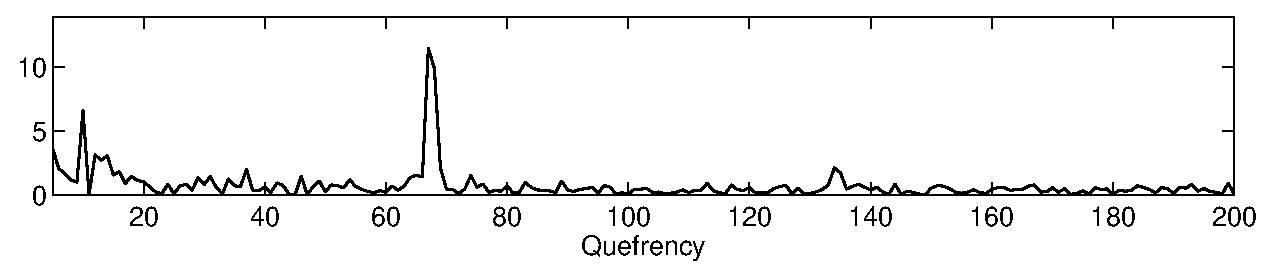
\includegraphics[scale=.6]{DCT_cepstrum_voiced_clean.eps}}
    \caption[Using cepstrum for pitch estimation]{Using cepstrum for pitch estimation: \subref{Fig:logspectrum_voiced} the log-spectrum of a sample voiced frame and \subref{Fig:cepstrum_voiced} its cepstrum, showing a distinct spike corresponding to its pitch.}
    \label{Fig:DFT_voiced_frame_clean}
\end{figure}

Some researchers have used the Mel-frequency cepstral coefficients (MFCC) as the input feature to a supervised classifier for the speech/non speech detection \cite{kinnunen2007voice,martin2001robust,cho2011enhanced}.
%Each MFCC vector is often appended with its delta and double-delta coefficients, result in a 36-dimensional feature space.
Kunnunen \etal \cite{kinnunen2007voice} used a feature vector consists of MFCC and its delta and double-delta coefficients to apply to a pre-trained discriminative model.
Fukuda \etal \cite{fukuda2008phone} proposed using Mel-frequency delta cepstral coefficients alone for VAD.
Delta cepstrum is defined as the first-order derivative of the cepstral sequence, and is widely used in speaker recognition systems.
This feature is sometimes referred to as `dynamic features' due to the fact that it can capture the dynamic changes between the cepstral frames.
Formally, delta cepstrum is derived as the following \cite{fukuda2008phone}:
\begin{equation}\label{eq:delta_cepstrum}
	\vt{\Delta c}_k = \sum_{i=1}^M k \left( \vt{c}_{k+i} - \vt{c}_{k-i} \right) / \left(2\sum_{i=1}^M i^2 \right)
\end{equation}

In \eq{delta_cepstrum}, a delta window of length $2M+1$ frames is used to extract the delta cepstrum vector $\vt{\Delta c}_k$ at time $k$.
In standard ASR systems, the value of $M$ is often set from two to four, depending on the frame size, frame rate and other parameters.
The bigger value of $M$ results in the wider temporal information across the consecutive cepstral frames being captured.
The effects of such long-term window for feature extraction will be studied more in a later section.

%Static harmonic feature in Mel-cepstrum domain: \cite{fukuda2010long}
Another technique has been proposed by Fukuda \etal \cite{fukuda2010long} to enhance the harmonic structure of the speech by performing filtering in the cepstral domain, a process usually referred to as \emph{liftering}.
This method assumes that pitch information containing the harmonic structure is included in the middle-range cepstra.
By filtering out the lower and higher cepstra, which are more likely to be corrupted by noise, the harmonic structure of the spectrum is enhanced.
The results reported show a great improvement in term of noise robustness in very low SNR situations of 0 dB to -5 dB.

\subsection{Harmonicity-based features}
One of the most powerful heuristic-based features for VAD is the harmonicity of the speech signal \cite{rabiner1978digital}.
It is well known that voiced speech has a unique structure, which contains multiple harmonics of the fundamental frequency $F_0$.
Unlike unvoiced speech, whose characteristics are easily confusable with such as car, wind and fan noise, the harmonic structure of voiced speech are preserved even in very noisy condition \cite{rabiner1978digital,kristjansson2005voicing}.
Observation from \fig{spectrum_snr0_whitenoise} shows that the most distinguishable harmonics under very noisy environments are around the first formant, which contains the highest energy.
However, this is not the case under certain noise types such as engine noise and babble noise (\fig{babble_-5db}), where the loudest noisy frequency range might happen to cover the first formant.
In this case, exploiting the harmonics in other frequency ranges might be more beneficial.


\begin{figure}[hh] %[hb] to put it to the bottom of the page
    \centering
    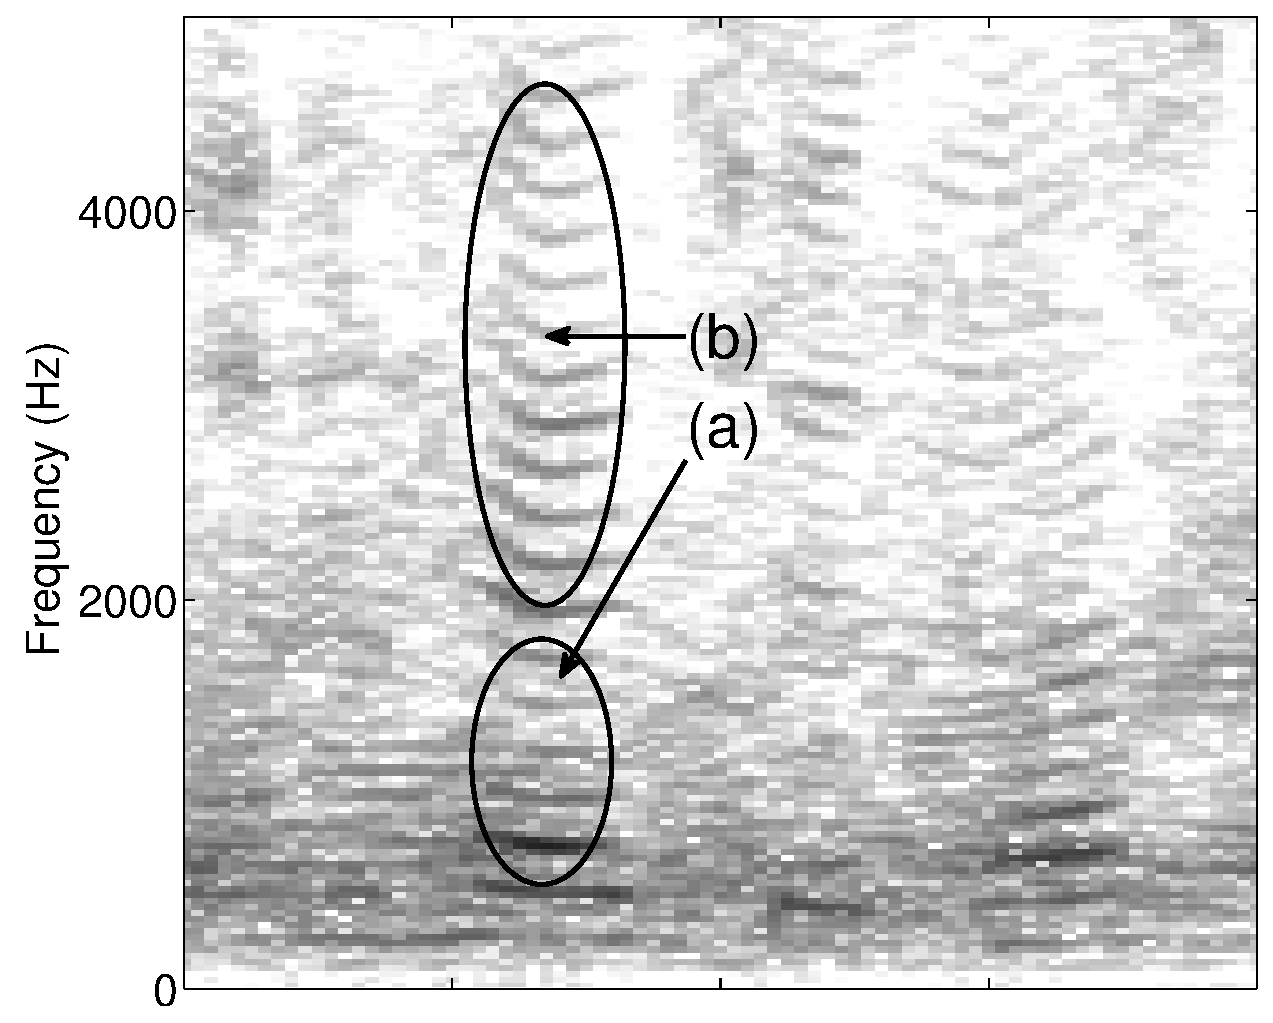
\includegraphics[width=0.5\textwidth]{babble_-5db.eps}            %Adjust width to taste
    \caption[A sample spectrum of speech corrupted by babble noise at SNR=$-5$dB]{A sample spectrum of speech corrupted by babble noise at SNR=$-5$dB. While the harmonics around the first formant (a) is destroyed, those in the higher frequency range (b) is still distinguishable.}
    \label{Fig:babble_-5db}        %For referencing in the text
\end{figure}


Harmonic structure in human speech is hard to exploit statistically.
Thus, most existing algorithms rely on heuristic cues to extract the periodicity feature of speech.
This is sometimes tied to the voiced/unvoiced classification and pitch detection problems, which often involves the estimation of the fundamental frequency $F_0$ \cite{ishizuka2006study}.
A number of earlier research focused on the auto-correlation of the signal to search for self-repetition components from the signal \cite{rabiner1977use,kristjansson2005voicing}.
This includes the \emph{Maximum Autocorrelation Peak} \cite{kingsbury2002robust}, which finds the magnitude of the maximum peak within the range of lags that correspond to the range of pitch of male and female voices (50Hz--400Hz).
Another measure is the \emph{Autocorrelation Peak Count} \cite{basu2003linked}, which counts the number of peaks found in a range of lags.
Formally, the autocorrelation vector, $\vt{r}_k = \left[ r_{k,1} \dots r_{k,N} \right]^T$, of the $k$-th frame $\vt{x}_k$, and the estimated pitch, $\hat{f}_0$ are found as follow:
\begin{align}
    r_{k,\tau} &= \sum_{m=\tau}^N x_{k,m}x_{k,m-\tau} \\
    \tau_{max} &= \argmax{\tau} r_{k,\tau}      \\
    \hat{f}_0 &= f_s/\tau_{max}
\end{align}
Under environments that contain repetitive noise such as motor and car noise, auto-correlation-based features would fail because the loudest frequency component is usually the noise itself.
This leads to the motivation for more noise-robust techniques in the spectral and cepstral domains.

%In the spectral domain, repetitive noise components appear as spectral peaks. Simple spectral techniques such as filtering and average noise estimation can easily reduce the effect of such noise.

The harmonic structure of the voiced speech appears in the spectrum as a train of spectral peaks, each of which is in multiple of the fundamental frequency.
A common approach to capture this structure is by using comb filtering techniques \cite{tolba1998robust} and the alikes \cite{ishizuka2006study}.
A comb filter consists of a series of regularly spaced spikes in the frequency spectrum, causing constructive interference to the speech harmonics and destructive interference to all other frequency components.
In practice, comb filters are used to `search' for the fundamental frequency by setting its lags between the comb spikes to the possible frequencies.
A matched frequency would give a high correlation with the signal in the spectral domain.

Under high noise environments, however, comb filter approaches appear to be not reliable.
In these cases, noise components usually corrupt most speech harmonics and causing false spikes across the spectrum, which results in the inaccurate pitch estimation and leads to the degradation of VAD performance (\fig{babble_-5db}).
To make it more robust in high noise environments, it is essential to perform enhancement procedures to possibly restore the spikes of the speech harmonics and reduce those of noise. Ichikawa \etal \cite{ichikawa2008local} proposed a technique that does not involve the estimation of $F_0$, named the \emph{Local Peak Enhancement} (LPE).
The method operates in the cepstral domain, which filters out the cepstra that are more likely to belong to noise (upper and lower range) and reserves those that cover the possible harmonic structures in the human voice (middle range).
According to the authors the peak enhancement can achieve its optimal performance by combining with noise reduction procedures such as Wiener Filter \cite{papoulis2002probability} and spectral subtraction techniques \cite{boll1979suppression}.

Most harmonicity-based techniques mentioned above would suffer in environments containing cross-talk speech, such as babble noise or overlapped speaking.
Indeed, the interference of other speakers causes the spectral frames of voiced speech to possibly contain more than one fundamental frequencies, which causes great confusion to the estimator.
To address this problem, another measure in the spectral domain was proposed by Krishnamachari \etal \cite{krishnamachari2000spectral}, named the \emph{Spectral Autocorrelation Peak Valley Ratio} (SAPVR), which takes the autocorrelation of the magnitude spectrum and uses the ratio between the peak and valley of the first local maximum as the harmonicity measure.
By finding the local maximum peak in the spectral autocorrelation domain, the method effectively removes the spectral peaks caused by the overlapped speech.
However, the proposed technique was studied in a clean co-channel with overlapping speech from two speakers; there has not been much research on applying it to noisy environments such as babble noise.

%\subsection{Entropy}
One of the few statistical approaches to exploit the harmonicity of voiced speech for speech detection is the spectral entropy \cite{krishnamachari2000spectral,shen1998robust,huang2000novel,basu2003linked}.
By interpreting the short-time spectrum $X_k$ as discrete random variable, its entropy, according to Shannon's information theory, can measure the randomness of the frame.
Due to the harmonic structure of voiced speech, it is expected that the voiced speech will have lower entropy than that of noise and unvoiced frame.
Shen \etal \cite{shen1998robust} first proposed an entropy measure for VAD using a set of pre-trained weight factors for adjusting the different contribution of the frequencies across the spectrum:
\begin{align}
    p(X_{k,i}) &= X_{k,i} / \sum_{j=1}^L X_{k,j} \\
    h_k &= - \sum_{i=1}^L w_i p(X_{k,i}) \log p(X_{k,i})
\end{align}
where $p(X_{k,i})$ is a probability measure of spectral distribution of the $i$-th frequency bin of the $k$-th spectral frame; and $w_i$ is the weight factor of the $i$-th frequency bin, statistically pre-estimated from training data.
According to Huang and Yang \cite{huang2000novel}, using spectral entropy feature alone cannot distinguish speech from periodic background noise such as babble noise and music.
The authors proposed to combine this feature with the energy measure as a compromise in cases where background noise have strong harmonic structure but its energy is still less than that of speech:
\begin{equation}
    \operatorname*{EE-Feature}(\vt{x}_k) = \sqrt{1+ \left|(\operatorname*{Energy}(\vt{x}_k) - E_0)(h_k - h_0) \right|}
\end{equation}
where $E_0$ and $h_0$ are the estimated energy and entropy of recent non-speech frames, which are subtracted from the current frame measures to reduce the effects of noise.
Reported result showed an improvement over using energy or entropy feature alone.
Unfortunately, it was only tested with recordings at SNR=15 dB; no further experimental result has been used to confirm its robustness under lower SNR conditions.
Nevertheless, this feature combination has a reasonably low complexity, which can be easily implemented in hardware applications, such as in-car entertainment systems; while its robustness can be compromised by using close-talk microphones to achieve a sufficient SNR level.


%spectral tracking

%eg. ETSI-AMR VAD

\subsection{Long-term features}
%Describes the existing long-term features.

%Linear Dynamic Model
%Summary of the aforementioned features, why no single feature could be robust in all scenarios, each feature fail on a certain noise condition.

%Most of the aforementioned techniques rely on the short-term statistics of the signal to distinguish speech and noise. These techniques assume that speech is stationary over short periods of 20ms, while noise
%By assuming that speech is stationary over short periods of 20ms, the signal is divided in to frames of observation, from which the signal is analyzed independently to determining their speech/non-speech category.

Human speech is well known as a non-stationary signal.
A person with average speaking rate produces approximately 10--15 phonemes per second \cite{liberman1996speech}, each of which has different statistics, causing the statistics of speech to vary greatly over time.
On the other hand, most noise encountered in everyday conversation are stationary (white noise, machinery noise), or at least their degrees of varying are much lower than speech's (car noise, babble noise).
This suggests that the analysis over a longer window for exploiting the degree of non-stationarity of the signal might be beneficial for distinguishing speech from noise.

Long-term temporal information has been the focus of research in the speech community recently \cite{chen2004learning,fukuda2008short,hermansky1999temporal}.
Psychophysical study \cite{poeppel2003analysis} also showed that temporal information from both short windows (20--40ms) and long windows (150--250ms) are important to understand spoken language.
For VAD, most techniques exploit the long-term information by either extending the processing windows \cite{ramirez2004efficient} or performing post-processing over the features extracted from a set of contiguous frames \cite{fukuda2008phone,ghosh2011robust}.
Ramirez \etal \cite{ramirez2004efficient} finds the long-term spectral envelope, from which a measure is derived from the sub-band SNRs (Equations \ref{eq:LTSD} and \ref{eq:LTSE}).
Fukuda \etal \cite{fukuda2008phone,fukuda2008short,fukuda2010long} proposed the long-term dynamic feature for VAD, derived from fusing the delta cepstrum of the $2K+1$ neighbor frames (\eq{delta_cepstrum}).
Ghosh \etal \cite{ghosh2011robust} calculate the variance of the long-term sub-band entropies, showing a great improvement in both stationary and non-stationary noise conditions:
\begin{align}
    \mathcal{L}_k &= \operatorname*{Var}(\xi)         \\
    \xi &= \sum P(k) \log P(k)                      \\
    P(k) &= \frac{|X_{k,i}|^2}{\sum |X_{k,j}|^2}
\end{align}

Frankel \cite{frankel2003linear} proposed the \emph{Linear Dynamic Models} to exploit the long-term information in a more sophisticated mathematical framework, which has been applied to VAD and reported state-of-the-art results by Kannu \etal \cite{kannu2011linear}. (\emph{To be extended})

\subsection{Summary}
This section have reviewed the many classes of features that have been proposed in the literature. Each of these classes of features have shown certain advantages and disadvantages when applied to the problem of voice activity detection, in which the main goal is to maximize the discriminative power and noise robustness. Energy-based features is simple and can be easily implemented in hardware applications, but they are not noise robust. Domain-specific features such as those derived from the spectrum and cepstrum are beneficial from a wide class of filtering techniques to reduce the effects of noise. Under very low SNR conditions such as below 0 dB, however, most statistical information in the spectral and cepstral domains are badly affected. In these cases, using the heuristic cues, such as the harmonicity characteristics of the voiced speech seems to be the most robust way to distinguish speech from noise.
Finally, including the long-term temporal information of the signal can exploit the different degrees of variability of speech and noise, which results in an improved discriminative power of the features.

%The process of feature extraction for VAD is related to many other fields of speech processing research such as speech recognition, speech enhancement, pitch estimation and noise reduction. In some cases, their performance are mutually dependent. For example, harmonicity-based features rely on the good results achieved from the pitch estimation or speech enhancement process, while the spectral features usually require the noise estimation and reduction to be done accurately. Techniques proposed in one field can share their result in the other. Such as the MFCC features, the most widely used in speech recognition, show acceptable results in most normal noise conditions. Or the Linear Dynamic Models, originally developed for speech recognition,
%The feature extraction process can be seen as finding an appropriate representation for the speech signal, either by transforming to different domains such as the spectrum or cepstrum, or by its heuristically-based characteristics.
